
\section{GraphML}
\prc

\textit{GraphML} ist ein einfaches Dateiformat das für die Erstellung von Graphen genutzt werden kann. Dabei handelt es sich um eine Grundlage die die strukturellen Eigenschaften eines Graphen beschreiben kann. Die unterstützten Grundlagen laut \cite{graphml} sind:

\begin{itemize}
	\item gerichtete, ungerichtete und gemischte Graphen
	\item Hypergraphen
	\item hierarchische Graphen
	\item Referenzen auf externe Daten
	\item Applikationsspezifische Attribut-Daten und
	\item light-weight Parser
\end{itemize}

\noindent
Das Dateiformat basiert auf XML was es einfach macht damit Graphen zu generieren, archivieren und entwickeln.

\subsection{Hintergrund}

Die Entwicklung von GraphML während eines Workshops auf der Graph Drawing Symposium im Jahre 2000 in Williamsburg. Ein erster Ansatz für das Endergebnis wurde auf der Graph Drawing Symposium, 2001 in Wien vorgestellt \footfullcite{graphml}.
\\

\noindent
Seither wurden laufend Erweiterungen erstellt und auch Anwendungen die auf diesem Dateiformat aufbauen. Eine dieser Anwendungen ist das in Kapitel \ref{yed} beschriebene Programm yEd. Die folgenden Kapitel beziehen sich auf das modifizierte GraphML Format für yEd.

\subsection{Grundelemente und Aufbau}

Aufgrund der Eigenschaft, dass es sich bei GraphML um ein XML-Dokument handelt ist der Aufbau übersichtlich und man kann mit nur vier Elementen einen ganzen Graphen beschreiben \footfullcite{graphmltutorial}. Zu diesen vier Elementen gehören:

\begin{itemize}
	\item Das \textit{graphml}-Element, dass das \textit{root}-Element des Graphen bildet.
	\item Das \textit{graph}-Element, dass den Graphen kennzeichnet.
	\item Das \textit{node}-Element, dass einen Knoten des Graphen widerspiegelt.
	\item Das \textit{edge}-Element, dass die Kanten zwischen den Knoten repräsentiert.
	\\
\end{itemize}

\noindent
Innerhalb des \textit{graph}-Elements sind die Elemente für die Knoten und Kanten des Graphen angesiedelt. Hierbei muss aber nicht auf die Reihenfolge der Elemente geachtet werden.

\subsection{Generierung der Datei und Aufbau}

Um einen GraphML-Datei für yEd zu erstellen bietet yWorks, die Entwickungsfirma der Applikation, eine APi mit dem Namen yFiles an. Diese kann man aber nur für Java, JavaFX, .NET, WPF und HTML verwenden. Weil wir als Diplomarbeitsteam uns dazu entschieden haben \textit{Pyhton} als Programmiersprache zu verwenden stieß man hierbei schon auf die ersten Probleme. 
\\

\noindent
Jedoch konnte durch den Aufbau der Datei als XML und durch reverse Engineering, der Graph in Form von XML als Text in eine Datei geschrieben werden. Dementsprechend wurde ein Konvertierer entwickelt der die Informationen der XERML-Datei sinngemäß in eine GraphML-Datei umwandelt, damit hinterher ein vollständiges ER-Diagramm erstellt wird.

\subsubsection{Initiierung der Datei}

Damit die Datei von yEd korrekt gelesen werden kann müssen auch die entsprechenden \textit{Namensräume} für das XML gesetzt werden. Zudem werden von yEd in der GraphML-Datei \textit{key-Elemente} verwendet um den Knoten und Kanten innerhalb des Graphen den richtigen Typ zuweisen zu können. Bei der Initiierung wird zudem noch das Root-Element der GraphML-Datei erstellt. Hierbei ist anzugeben ob es sich bei dem Graphen um einen gerichteten, ungerichteten oder gemischten Graphen handelt. Für den gewählten Ansatz wird ein gerichteter Graph erstellt, weil dies auch die gewählte Einstellung von yEd ist bei der Erstellung eines ER-Diagramms, wie sich durch reverse Engineering herausgestellt hat.
\\

\noindent
Der XML-Code bis nach dem öffnen des \textit{graph}-Elements sieht also wie folgt aus:

\begin{lstlisting}[language=XML, label={xmlHeader}, caption={Header der GraphML-Datei mit nötigen Namensräumen}]
<?xml version="1.0" encoding="UTF-8" standalone="no"?>
<graphml xmlns="http://graphml.graphdrawing.org/xmlns"
	xmlns:java="http://www.yworks.com/xml/yfiles-common/1.0/java"
	xmlns:sys="http://www.yworks.com/xml/yfiles-common/markup/primitives/2.0" 
	xmlns:x="http://www.yworks.com/xml/yfiles-common/markup/2.0"
	xmlns:xsi="http://www.w3.org/2001/XMLSchema-instance"
	xmlns:y="http://www.yworks.com/xml/graphml"
	xmlns:yed="http://www.yworks.com/xml/yed/3"
	xsi:schemaLocation="http://graphml.graphdrawing.org/xmlns
	http://www.yworks.com/xml/schema/graphml/1.1/ygraphml.xsd">
<key for="node" id="d1" yfiles.type="nodegraphics"/>
<key for="edge" id="d2" yfiles.type="edgegraphics"/>
<graph edgedefault="directed" id="G">
\end{lstlisting}

\subsubsection{Erstellung der Knoten und Kanten}
\prc

Die Informationen für die Erstellung der Knoten und Kanten werden aus einem ,,\textit{etree}'' ausgelesen der zuvor mithilfe der XERML-Datei des Benutzers erstellt wird. Beim Konverter werden diese Informationen dann analysiert und in ein entsprechendes Format für die GraphML Datei umgewandelt.

\subsubsubsection{Knoten}

\noindent
Beim Schreiben des XML-Codes für die Knoten wird ein Element für einen Knoten mit einer \textit{ID} als Attribut angelegt. Mithilfe dieser ID können später die Kanten zwischen den Knoten gezeichnet werden. Innerhalb des Knotenelements sind ein \textit{data-Element}. Diese zwei XML-Elemente gehören zu den grundlegenden GraphML-Elementen. Die spezifische Information über dem Knoten, den man am Ende im ER-Diagramm sieht, steht im \textit{GenericNode} der ein Kindelement von dem data-Element ist. 
\\

\noindent
In der folgenden Strukturbeschreibung sieht man wie ein Knoten in GraphML für die Verwendung mit yEd aufgebaut ist. Man beachte jedoch, dass Attribute mit Standardwerten beim Element \textit{NodeLable} weggelassen wurden, weil diese ohnehin nicht  beeinflusst werden.

\begin{verbatim}
Element: node
|
+-- Attribut: id
+-- Element: data
    |
    +-- Attribut: key
    +-- Element: y:GenericNode
        |
        +-- Attribut: configuration
        +-- Element: y:Geometry
            |
            +-- Attribut: heigth
            +-- Attribut: width
            +-- Attribut: x
            +-- Attribut: y
        +-- Element: y:Fill
            |
            +-- Attribut: hasColor
            +-- Attribut: color
            +-- Attribut: transparent
        +-- Element: y:NodeLable
        +-- Element: y:StyleProperties
            |
            +-- Element: y:Property
                |
                +-- Attribut: class
                +-- Attribut: name
                +-- Attribut: value
\end{verbatim}
\prc

\noindent
Diese Struktur ist aber nicht immer gleich. Zum Beispiel wird das Element \textit{StyleProperties} nur als Kindelement von Node angeführt, wenn es sich bei dem Knoten um einen schwachen Entitytypen handelt. Weiteres ist das Attribut \textit{color} nur dann gesetzt, wenn der Benutzer sein ER-Diagramm farbig haben möchte. 
\\

\noindent
Im nachfolgenden XML-Beispiel sieht man wie der Entitytyp ,,Person'' aus dem Datenmodell Schulinformationssystem aussieht, wenn dieser nicht färbig dargestellt wird:

\begin{lstlisting}[language=XML, caption=Entitytyp Person dargestellt in GraphML, label={xmlTypen}]
<node id="n0">
	<data key="d1">
		<y:GenericNode configuration="com.yworks.entityRelationship.small_entity">
			<y:Geometry height="50.0" width="90.0" x="285.0" y="135.0"/>
			<y:Fill hasColor="false" transparent="false"/>
			<y:NodeLabel alignment="center" autoSizePolicy="content"
				fontFamily="Dialog" fontSize="12" fontStyle="plain"
				height="17.96875" horizontalTextPosition="center"
				iconTextGap="4" modelName="internal" modelPosition="c"
				textColor="#000000" verticalTextPosition="bottom"
				visible="true">Person</y:NodeLabel>
		</y:GenericNode>
	</data>
</node>
\end{lstlisting} 

\noindent
Wie man ebenfalls anhand des Beispieles sehen kann, wird in Zeile 3 durch das Attribut \textit{configuration} der Typ des Knoten festgelegt. Bei der Erstellung eines ER-Diagramms werden im gegebenen Sachzusammenhang zwischen 3 Typen unterschieden:
\\

\begin{itemize}
	\item \begin{verbatim}small_entity\end{verbatim}
	- für einen Entitytyp
	\item \begin{verbatim}relationship\end{verbatim}
	- für einen Beziehungstyp
	\item \begin{verbatim}attribute\end{verbatim}
	- für ein Attribut
	\\
\end{itemize}

\noindent
Abhängig vom Typ der an jener Stelle angeführt ist, wählt yEd eine andere Form um den Knoten darzustellen. Wie der Knoten aus dem Beispiel aussieht, kann man in Abbildung \ref{entityPerson} sehen.

\begin{figure}[!h]
	\begin{center}
		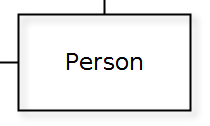
\includegraphics[width=6cm]{images/entityPerson.png}
		\caption{Entitytyp Person dargestellt in yEd}
		\label{entityPerson}
	\end{center}
\end{figure}

\subsubsubsection{Kanten}
\prc

\noindent
Die Kanten werden in einer GraphML-Datei über ein \textit{edge-Element} beschrieben. Dieses Elemen,t enthält genauso wie auch schon das node-Element eine ID, zusätzlich bekommt es jedoch die Attribute \textit{source} und \textit{target} die als Werte jene IDs der Knoten erhalten, die diese Kante zusammenhalten soll.
\\

\noindent
Wie auch schon bei den Knoten werden in der folgenden Strukturbeschreibung für die Kanten in einer GraphML-Datei all jene Attribute und Elemente beim Element \textit{EdgeLable} weggelassen, die mit Standardwerten initiiert sind.

\begin{verbatim}
Element: edge
|
+-- Attribut: id
+-- Attribut: source
+-- Attribut: target
+-- Element: data
    |
    +-- Attribut: key
    +-- Element: y:PolyLineEdge
        |
        +-- Element: y:LineStyle
            |
            +-- Attribut: color
            +-- Attribut: type
            +-- Attribut: width
        +-- Element: y:Arrows
            |
            +-- Attribut: source
            +-- Attribut: target
        +-- Element: y:EdgeLable

\end{verbatim}

\noindent
Dadurch das der Benutzer von ERMTK sich bei der Generierung einer GraphML-Datei entscheiden kann ob er sein ER-Diagramm in der Crow-foot Notation oder in der (min,max)-Notation, fällt bei der Crow-foot Notation das Element EdgeLable weg.
\\

\noindent
Im folgendem XML-Beispiel sieht man die Kante die den Entitytypen ,,Person'' mit dem Beziehungstypen ,,ist Elternteil von'' verbindet:

\begin{lstlisting}[language=XML, caption=Kante zwischen einem Entitytypen und einem Beziehungstypen, label={xmlKanten}]
<edge id="e26" source="n0" target="n19">
	<data key="d2">
		<y:PolyLineEdge>
			<y:LineStyle color="#000000" type="line" width="1.0"/>
			<y:Arrows source="none" target="none"/>
			<y:EdgeLabel alignment="center" configuration="AutoFlippingLabel"
				distance="2.0" fontFamily="Dialog" fontSize="12"
				fontStyle="plain" hasBackgroundColor="false"
				hasLineColor="false" height="17.96875"
				horizontalTextPosition="center" iconTextGap="4"
				modelName="custom" preferredPlacement="source_right"
				ratio="0.5" textColor="#000000" verticalTextPosition="bottom"
				visible="true" width="90.3203125" x="-15.16015625"
				xml:space="preserve" y="-22.94091796875003">
				(0,n)
				<y:LabelModel>
					<y:SmartEdgeLabelModel autoRotationEnabled="false" defaultAngle="0.0"
						defaultDistance="10.0"/>
				</y:LabelModel>
				<y:ModelParameter>
					<y:SmartEdgeLabelModelParameter angle="0.0"
						distance="30.0" distanceToCenter="true" position="right" ratio="0.0" 
						segment="0"/>
				</y:ModelParameter>
			<y:PreferredPlacementDescriptor angle="0.0"
				angleOffsetOnRightSide="0" angleReference="absolute"
				angleRotationOnRightSide="co" distance="-1.0"
				placement="source" side="right"
				sideReference="relative_to_edge_flow"/>
			</y:EdgeLabel>
		</y:PolyLineEdge>
	</data>
</edge>
\end{lstlisting}

\noindent
Wie man in der 1. Ziele des Beispiels erkennen wird dort die Information gespeichert welche Knoten verbunden werden. Dies wird dann in yEd wie in der Abbildung \ref{yedKante} dargestellt.

\begin{figure}[!h]
	\begin{center}
		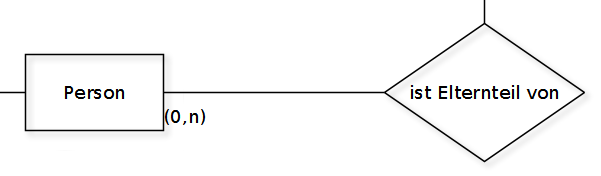
\includegraphics[width=10cm]{images/yedKante.png}
		\caption{Entitytyp Person dargestellt in yEd}
		\label{yedKante}
	\end{center}
\end{figure}

\subsection{Python-Code für die Generierung}

Um die GraphML-Datei für yEd zu erstellen, wurde die Klasse \textit{GraphmlConverter} geschrieben die den Inhalten der XERML-Datei in das richtige Format bringt und in eine Datei schreibt.
\\

\noindent
Zu Beginn wird die Datei, die später mit yEd geöffnet werden soll erstellt. Dazu wird der Parameter \textit{output} abgefragt, den der Benutzer angeben kann. Je nach Angaben des Benutzers wird die Datei an dem momentanen Pfad mit dem Namen \textit{output.graphml} erstellt an dem der Benutzer den Befehl ausgeführt hat oder er gibt einen Pfad mit Namen an, andem die Datei erstellt werden soll. Der Codeausschnitt \ref{createFile} behandelt diesen Fall:


\begin{lstlisting}[language=Python,label={createFile},caption={Codeausschnitt für die Erstellung der GraphML-Datei}]
try:
	if args.output is None:
		if os.path.exists("output.graphml"):
			os.remove("output.graphml")
		self.out = open("output.graphml", "w+")
	else:
		if os.path.exists(os.getcwd() + "/" + args.output):
			os.remove("./" + args.output)
		self.out = open(os.getcwd() + "/" + args.output, "w+")
	self.init_file()
except IOError:
	print(Fore.RED + "There was a Problem creating the file. Please try again" + Fore.RESET)
	return
\end{lstlisting}

\prc
\noindent
Wie man in Zeile 10 von \ref{createFile} sieht, wird dort die Funktion \textit{init\_file()} aufgerufen. In dieser Funktion wird die Datei soweit vorbereitet, dass der XML-Code für die Entity- und Beziehungstypen \ref{xmlTypen} und für die Kanten \ref{xmlKanten} hineingeschrieben werden kann. Der XML-Code der dabei hineingeschrieben wird ist in Listing \ref{xmlHeader} zu sehen.
\\

\noindent
Anschließend wird in einem XML-Baum der die Informationen aus der XERML-Datei enthält nach den Entity- und Beziehungstypen gesucht damit auch diese ihren Weg in die GraphML-Datei finden. Dieser Vorgang wird in dem Listing \ref{searchElements} vereinfacht dargestellt. Vereinfacht bedeuted in diesem Sinne, dass \textit{if}-Anweisungen, \textit{for}-Schleifen, und Definitionen von Variablen sowie deren Verwendung bei den Funktionsaufrufen weggelassen werden, damit die Logik des Codes im Vordergrund steht. Die komplette Darstellung des Codes kann man im Anhang finden.
\\

\begin{lstlisting}[language=Python, label={searchElements}, caption={Vereinfachter Code zum hizufügen der Entity- und Beziehungstypen}]
root = self._tree.getroot()
#------------------------------------------------------------------------------------------------------
for child in root:
	if child.tag == "ent":
		self.create_node()
		if args.attr:
			for attr in child:
				self.create_attribute()
#------------------------------------------------------------------------------------------------------
	elif child.tag == "rel":
		for part in child:
			if part.tag == "part":
				self.create_node()
#------------------------------------------------------------------------------------------------------
				if args.notation == "crowfoot":
					# Die folgende if-Anweisung wird betreten wenn ein fuer beide Kantenenden ein Knoten definiert ist
					if key_e != "" and key != "":
						self.create_edge()
					else:
						print(Fore.RED + "There was an entity missing for a relationship" + Fore.RESET)
				else:
					# Die folgende if-Anweisung wird betreten wenn ein fuer beide Kantenenden ein Knoten definiert ist
					if key_e != "" and key != "":
						self.create_chen_edge()
					else:
						print(Fore.RED + "There was an entity missing for a relationship" + Fore.RESET)
#------------------------------------------------------------------------------------------------------
			elif part.tag == "super":
				if not generalization_node:
					generalization_node = True
					self.create_generalization_node()
					# Die folgende if-Anweisung wird betreten wenn ein fuer beide Kantenenden ein Knoten definiert ist
					if key_e != "" and key != "":
						if args.notation == "chen":
							self.create_chen_edge()
						else:
							self.create_edge()
					else:
						print(Fore.RED + "There was an entity missing for a relationship" + Fore.RESET)
#------------------------------------------------------------------------------------------------------
			elif part.tag == "sub":
				# Die folgende if-Anweisung wird betreten wenn ein fuer beide Kantenenden ein Knoten definiert ist
				if key_e != "" and key != "":
					if args.notation == "chen":
						self.create_chen_edge()
					else:
						self.create_edge()
				else:
					print(Fore.RED + "There was an entity missing for a relationship" + Fore.RESET)
			elif part.tag == "attr" and args.attr:
				self.create_attribute()
\end{lstlisting}
\prc

\noindent
Nachdem der vereinfachte Codeabschnitt \ref{searchElements} abgeschlossen ist, wird die GraphML-Datei ordnungsgemäß mit der Funktion \textit{close\_file()} geschlossen. Als letzten Schritt wird dem Benutzer noch mitgeteilt, wo sich die GraphML-Datei befindet, damit dieser sein ER-Diagramm in yEd inspizieren kann.




